\documentclass[10pt,a4paper,openright]{book}

%% Formateo del título del documento
\title{Topología elemental}
\author{Mario Calvarro Marines}
\date{}

%% Formateo del estilo de escritura y de la pagina
\pagestyle{plain}
\setlength{\parskip}{0.35cm} %edicion de espaciado
\setlength{\parindent}{0cm} %edicion de sangría
\clubpenalty=10000 %líneas viudas NO
\widowpenalty=10000 %líneas viudas NO
\usepackage[top=2.5cm, bottom=2.5cm, left=3cm, right=3cm]{geometry} % para establecer las medidas de los margenes
\usepackage[spanish]{babel} %Para que el idioma por defecto sea español
\usepackage{ulem} % para poder subrayar entornos especiales como las secciones

%% Texto matematico y simbolos especiales
\usepackage{amsmath} %Paquetes para mates
\usepackage{mathtools}
\usepackage{amsfonts} %Paquetes para mates
\usepackage{amssymb} %Paquetes para mates
\usepackage{stmaryrd} % paquete para mates
\usepackage{latexsym} %Paquetes para mates
\usepackage{cancel} %Paquete tachar cosas
\usepackage{accents} %Paquete acentos

%% Ruta de las fotos e inclusion de las mismas
\usepackage{graphicx}
\graphicspath{{./fotos/}}

%% Inclusion de referencias cruzadas por defecto y específicas
\usepackage{hyperref}

%% Paquete para definir y utilizar colores por el documento
\usepackage[dvipsnames,usenames]{xcolor} %activar e incluir colores
    %% definicion de los colores que se van a utilizar en cada cabecera
    \definecolor{capitulos}{RGB}{60,0,0}% gama de colores de los capitulos
    \definecolor{secciones}{RGB}{95,8,5}% gama de colores de las secciones
    \definecolor{subsecciones}{RGB}{140,36,31}% gama de colores de las subsections
    \definecolor{subsubsecciones}{RGB}{188,109,79}% gama de colores de las subsubsections
    \definecolor{teoremas}{RGB}{164,56,32}% gama de colores para los teoremas
    \definecolor{demos}{RGB}{105,105,105} % gama de colores para el cuerpo de las demostraciones

%% Paquete para la edición y el formateo de capítulos, secciones...
\usepackage[explicit]{titlesec}
    %% Definición del estilo de los capítulos, secciones, etc...
    \titleformat{\chapter}[display]{\normalfont\huge\bfseries\color{capitulos}}{}{0pt}{\Huge #1}[\titlerule]
    \titleformat{\section}{\normalfont\Large\bfseries\color{secciones}}{}{0pt}{#1}
    \titleformat{\subsection}{\normalfont\large\bfseries\color{subsecciones}}{}{0pt}{\uline{#1}}
    \titleformat{\subsubsection}{\normalfont\normalsize\bfseries\color{subsubsecciones}}{}{0pt}{#1}

%% Paquete para el formateo de entornos del proyecto
\usepackage{ntheorem}[thmmarks]
    %% Definicion del aspecto de los entornos matematicos del proyecto
    \theoremstyle{break}
    \theoremheaderfont{\normalfont\bfseries\color{teoremas}}
    \theorembodyfont{\itshape}
    \theoremseparator{\vspace{0.2cm}}
    \theorempreskip{\topsep}
    \theorempostskip{\topsep}
    \theoremindent0cm
    \theoremnumbering{arabic}
    \theoremsymbol{}
    \theoremprework{\vspace{0.2cm} \hrule}
    \theorempostwork{\vspace{0.2cm}\hrule}
        \newtheorem*{defi}{Definición}

    \theoremprework{\vspace{0.25cm}}
        \newtheorem*{theo}{Teorema}

    \theoremprework{\vspace{0.25cm}}
    	\newtheorem*{coro}{Corolario}

    \theoremprework{\vspace{0.25cm}}
    	\newtheorem*{lema}{Lema}

    \theoremprework{\vspace{0.25cm}}
    	\newtheorem*{prop}{Proposición}

    \theoremheaderfont{\normalfont}
    \theorembodyfont{\normalfont\color{demos}}
    \theoremsymbol{\hfill\square}
    	\newtheorem*{demo}{\underline{Demostración}:}

    \theoremheaderfont{\normalfont}
    \theorembodyfont{\normalfont}
    	\newtheorem*{obs}{\underline{Observación}:}
    	\newtheorem*{ej}{\underline{Ejemplo}:}

%% Definicion de operadores especiales para simplificar la escritura matematica
\DeclareMathOperator{\dom}{dom}
\DeclareMathOperator{\img}{img}
\DeclareMathOperator{\rot}{rot}
\DeclareMathOperator{\divg}{div}
\DeclareMathOperator{\inter}{Int}
\DeclareMathOperator{\adh}{Adh}
\DeclareMathOperator{\fr}{Fr}
\newcommand{\dif}[1]{\ d#1}

%% Paquete e instrucciones para la generacion de los dibujos
\usepackage{pgfplots}
\pgfplotsset{compat=1.17}
\usepackage{tkz-fct}
\usepgfplotslibrary{fillbetween}
\usepackage{tikz,tikz-3dplot}
\tdplotsetmaincoords{80}{45}
\tdplotsetrotatedcoords{-90}{180}{-90}
\usetikzlibrary{arrows}
    %% style for surfaces
    \tikzset{surface/.style={draw=blue!70!black, fill=blue!40!white, fill opacity=.6}}

    %% macros to draw back and front of cones
    %% optional first argument is styling; others are z, radius, side offset (in degrees)
    \newcommand{\coneback}[4][]{
        %% start at the correct point on the circle, draw the arc, then draw to the origin of the diagram, then close the path
        \draw[canvas is xy plane at z=#2, #1] (45-#4:#3) arc (45-#4:225+#4:#3) -- (O) --cycle;
    }
    \newcommand{\conefront}[4][]{
        \draw[canvas is xy plane at z=#2, #1] (45-#4:#3) arc (45-#4:-135+#4:#3) -- (O) --cycle;
    }
    
    \tikzset{middlearrow/.style={decoration={markings, mark= at position 0.5 with {\arrow{#1}},},postaction={decorate}}}
    
    \usetikzlibrary{decorations.markings}
    
    \newcommand{\AxisRotator}[1][rotate=0]{
    \tikz [x=0.25cm,y=0.60cm,line width=.2ex,-stealth,#1] \draw (0,0) arc (-150:150:1 and 1);
    }
    
    \usetikzlibrary{shapes}


\begin{document}
\maketitle
\setcounter{tocdepth}{3}% para que salgan las subsubsecciones en el indice
\tableofcontents
\chapter{Espacios topológicos}%
\label{cha:espacios_topologicos}

\section{Conjuntos abiertos}%
\label{sec:conjuntos_abiertos}
\begin{defi}
Una \underline{topología} en un conjunto $X$ es una colección $\mathcal{T} \subset \mathcal{P}\left( x \right)$ de subconjuntos tal que:
\begin{enumerate}
    \item $\emptyset, X \in \mathcal{T}$ 
    \item Las uniones arbitrarias de elementos de $\mathcal{T}$ están en $\mathcal{T}$.
    \item Las intersecciones \underline{finitas} de elementos de $\mathcal{T}$ están en $\mathcal{T}$.
\end{enumerate}
Se dice que $\left( X, \mathcal{T} \right)$ es un \underline{espacio topológico}, los elementos de $\mathcal{T}$ se llaman \underline{abiertos} y los elementos de $X$ se llaman \underline{puntos}. 
\end{defi}

\begin{ej}
\begin{enumerate}
    \item \label{ejemplos_topologia:first} $\mathcal{T} = \{\emptyset, X\}$ es la topología \underline{trivial}; $\mathcal{T} = P\left( X \right)$, topología \underline{discreta}: si los puntos $\{x\} \in \mathcal{T}$, entonces cualquier $A = \bigcup_{x \in A} \{x\}$ es abierto.
    \item $\mathbb{R}^n$ con la topología usual definida mediante las bolas euclídeas.
    \item Cualquier distancia $d$ define una topología mediante sus bolas abiertas, igual que se define la usual. \underline{Notación}: 
    \[
    B\left( a, \varepsilon \right) = \{d\left( a, x \right) < \varepsilon\},\ B\left[ a, \varepsilon \right] = \{d\left( a, x \right) \le \varepsilon \},\ S\left[ a, \varepsilon \right] = \{d\left( a, x \right) = \varepsilon\} 
    \]
    \item En un conjunto se pueden definir muchas topologías distintas (por ejemplo (\ref{ejemplos_topologia:first})) pero se puede asumir que solo ``parezcan'' distintas. Ya se sabe que la topología usual de $\mathbb{R}^n$ se puede definir mediante muchas distancias distintas.

    %TODO: Dibujo
    \begin{center}
        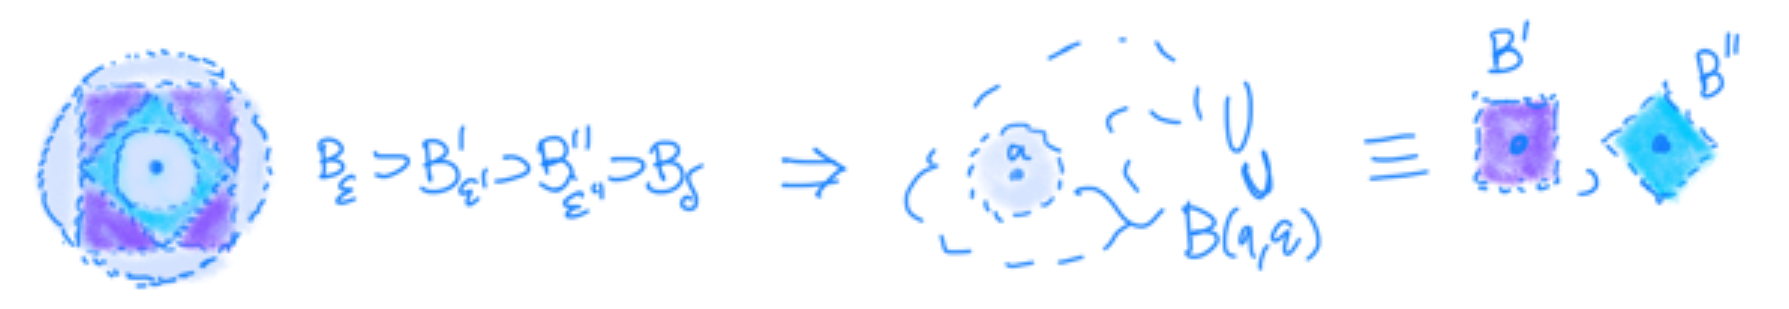
\includegraphics[scale=0.2]{images/topologia_metricas}  

        \textit{El dibujo representa distintas distancias\footnote{Procedentes de \textit{normas}.} en $\mathbb{R}^n$, pero todas definen la misma topología.} 
    \end{center}
    \item Una topología para ilustrar muchas propiedades (y contraejemplos). 

    Fijamos $a \in X$:
    \[
    \mathcal{T}_a = \{U \subset X: a \in U\} \cup \{\emptyset\} 
    \]
    La topología ``del punto''. El punto $\{a\}$ y todos los pares de puntos $\{a, x\}$ son abiertos. Se parece a la discreta pero difiere en que en esta última todos los puntos son abiertos.
\end{enumerate}
\end{ej}

\begin{defi}
Dos topologías $\mathcal{T}_1 \subset \mathcal{T}_2$ en $X$ se llaman \underline{comparables}: $\mathcal{T}_2$ es más ``fina'' que $\mathcal{T}_1$.
\end{defi}
Siempre se da:
\[
\mathcal{T}_{\text{trivial}} \subset \mathcal{T} \subset \mathcal{T}_{\text{discreta}} 
\]
Sea $\left( X, \mathcal{T} \right)$ un espacio topológico; a menudo se omite $\mathcal{T}$ ó el calificativo ``topológico''. 

\begin{defi}
\begin{enumerate}
    \item Un \underline{entorno abierto} de un punto $x \in X$ es un abierto $U$ que lo contiene. Se suele escribir $U^x$.
    \item Un \underline{entorno} de un punto $x \in X$ es un conjunto $V$ que contiene un abierto $U$ que contiene al punto. Se suele escribir $V^x$.\footnote{La intersección finita de entornos es entorno. (Si son abiertos es trivial)}
\end{enumerate}
\end{defi}
\begin{center}
    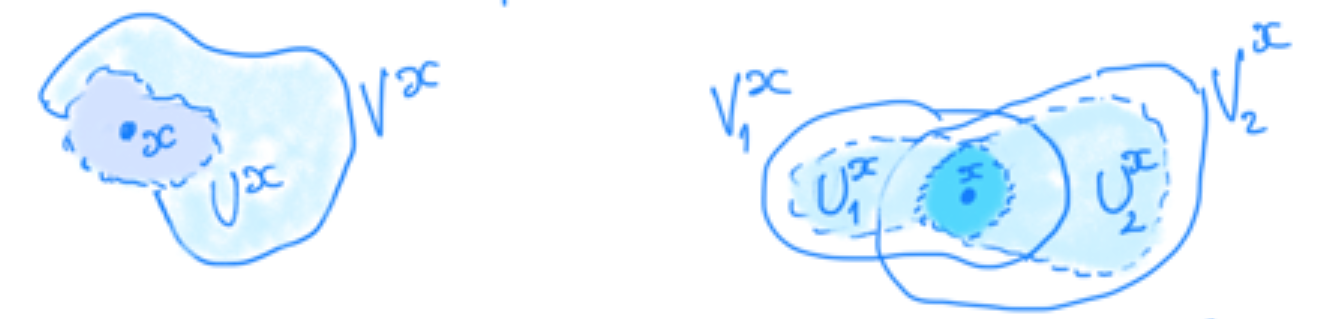
\includegraphics[scale=0.2]{images/def_entornos} 
\end{center}
\begin{obs}    
\begin{enumerate}
    \item \begin{align*}
        V_1^x \cap V_2^x &= V^x\\
        U_1^x \cap U_2^x &= U_{\text{ab}}^x \ni x
    \end{align*}

    %TODO: Corregir esta observación
    \item $U \in \mathcal{T}$ es entorno de todos \underline{sus} puntos.
    \begin{demo}
    \[
    x \in U \text{ abierto} \subset U
    \]
    \end{demo}
\end{enumerate}
\end{obs}

\begin{defi}
Sea $A \subset X$. Un \underline{punto interior de $A$} es un punto del que $A$ es entorno (luego $A$ lo contiene). El \underline{interior de $A$} es el conjunto de sus puntos interiores:
\[
\inter_X \left( A \right) = \mathring{A} = \{x \in A: \exists U_{\text{ab}}^x \subset A\} 
\]
\end{defi}
\begin{center}
    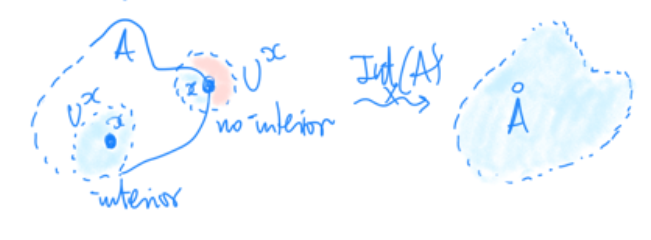
\includegraphics[scale=0.4]{images/def_interior} 
\end{center}

\begin{prop}
$\mathring{A}$ es el mayor abierto contenido en $A$: 
\[
\mathring{A} = \bigcup_{U^{ab} \subset A} U
\]
En particular, $A$ abierto $\Leftrightarrow A = \mathring{A} \Leftrightarrow A$ es un entorno de todos los puntos.    
\end{prop}
\begin{demo}
\begin{enumerate}
    \item $\mathring{A}$ es abierto: 
    \begin{gather*}
        \begin{rcases}
        \forall x \in \mathring{A} &\Rightarrow \exists U_{\text{ab}}^x \subset A\\
        \forall y \in U^x &\Rightarrow A \supset U^x \text{ es un abierto que contiene a } y \Rightarrow y \in \mathring{A}.\\
        \end{rcases} \Rightarrow U^x \subset \mathring{A}\\
        \Rightarrow \mathring{A} = \bigcup_{x \in \mathring{A}} U^x \text{ es abierto como unión de abiertos}
    .\end{gather*}
    \item $\mathring{A}$ es el mayor abierto contenido en $A$.
    \[
    U^{\text{ab}} \subset A \Rightarrow \forall x \in U^{\text{ab}} \subset A \Rightarrow x \in \mathring{A} \Rightarrow U \subset \mathring{A} 
    \]
\end{enumerate}
\end{demo}

\begin{ej}
\begin{enumerate}
    \item $\left( X, \mathcal{T}_{\text{trivial}} \right): A \neq X \Rightarrow A \not \supset X \Rightarrow \emptyset$ es el único abierto $\subset A \Rightarrow \mathring{A} = \emptyset$.

    \item En $\mathbb{R}^n$ con $\mathcal{T}_{\text{trivial}}$ ya lo sabemos bien:
    \[
    \inter\left( B\left[ a, \varepsilon \right] \right)  = B\left( a, \varepsilon \right);\ \mathring{\mathbb{Q}}^n = \emptyset;\ \mathring{\mathbb{Z}}^n = \emptyset
    \]
    \item Si $a \in X,\ \mathcal{T}_a : \mathring{\{a\}} = \{a\};\ x \neq a,\ \mathring{\{x\}} = \emptyset$.
\end{enumerate}
\end{ej}

\begin{prop}
\begin{enumerate}
    \item $A \subset B \Rightarrow \mathring{A} \subset \mathring{B}$.
    \item $\mathring{A} \cap \mathring{B} = \inter \left( A \cap B \right)$.
\end{enumerate}
\end{prop}
\begin{demo}
\begin{enumerate}
    \item $A \subset B \Rightarrow \mathring{A} \subset A \subset B$ y $\mathring{A}$ es abierto $\Rightarrow \mathring{A} \subset \mathring{B}$.
    \item 
    \begin{gather*}
    \begin{rcases}
    \begin{cases}
        \mathring{A} \cap \mathring{B} \text{ abierto (intersección finita de abiertos)}\\
        \mathring{A} \cap \mathring{B} \subset A \cap B 
    \end{cases} &\Rightarrow \mathring{A} \cap \mathring{B} \subset \inter \left( A \cap B \right)\\
    A \cap B \subset A, B \Rightarrow \inter \left( A \cap B \right) \subset \mathring{A}, \mathring{B} &\Rightarrow \inter\left( A \cap B \right) \subset \mathring{A} \cap \mathring{B}
    \end{rcases} \Rightarrow\\
    \boxed{\mathring{A} \cap \mathring{B} = \inter\left( A \cap B \right)} 
    .\end{gather*}
\end{enumerate}
\end{demo}

\section{Conjuntos cerrados}%
\label{sec:conjuntos_cerrados}
Sea $\left( X, \mathcal{T} \right)$ un espacio topológico.
\begin{defi}
Un conjunto \underline{cerrado} es un subconjunto $F \subset X$ tal que $U = X \setminus F$ es abierto.
\end{defi}
\begin{obs}
    Cerrado \underline{no} significa ``no abierto'', hay conjuntos que no son ni abiertos ni cerrados.
    \begin{center}
        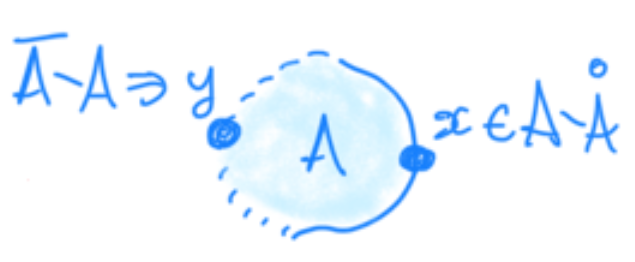
\includegraphics[scale=0.3]{images/def_cerrados} 
    \end{center}
\end{obs}
\begin{obs}
Se cumple:
\begin{enumerate}
    \item $X, \emptyset$ son cerrados.
    \item La intersección arbitraria de cerrados es cerrada.
    \item La unión finita de cerrados es cerrado.
\end{enumerate}
\begin{demo}
    Porque $\bigcap_{i \in  I} \left( X \setminus U_i \right) = X \setminus \bigcup_{i \in  I} U_i$ y $\bigcup_{i \in  I} X \setminus U_i = X \setminus \bigcap_{i \in  I} U_i$.
\end{demo}
\end{obs}

\begin{ej}
\begin{enumerate}
    \item En la topología trivial solo son cerrados $\emptyset$ y $X$. En la discreta, todos los subconjuntos son cerrados.
    \item En $\mathbb{R}^n$ con la topología usual ya sabemos todos los ejemplos: $B\left[ a, \varepsilon \right] : \lVert x - a \rVert \le \varepsilon$.
    \item Si $\mathcal{T}_1 \subset \mathcal{T}_2$, todo cerrado de $\mathcal{T}_1$ es cerrado de $\mathcal{T}_2$. 
\end{enumerate}
\end{ej}

Para saber cuándo se aleja un conjunto de ser cerrado tenemos:
\begin{defi}
Sea $A \subset X$. Un punto \underline{adherente} a $A$ es un punto cuyos entornos intersecan todos a $A$. La \underline{adherencia} de $A$ es el conjunto de sus puntos adherentes. 
\[
\adh_X\left( A \right) = \overline{A} = \{x \in X: \forall V^x \cap A \neq \emptyset\} 
\]
\end{defi}

\begin{obs}
Las primeras fórmulas importantes son:
\begin{gather*}
    \boxed{X \setminus \overline{A} = \inter\left( X \setminus A \right)} \\
    \boxed{X \setminus \mathring{B} = \overline{X \setminus B}} 
.\end{gather*}
\begin{demo}
\begin{itemize}
    \item $x \in X \setminus \overline{A} \Leftrightarrow x \not\in \overline{A} \Leftrightarrow \exists U^x \cap A = \emptyset \Leftrightarrow \exists U^x \subset X \setminus A \Leftrightarrow x \in \inter\left( X \setminus A \right)$
    \item $x \not\in \mathring{B} \Leftrightarrow \not\exists U^x \subset B \Leftrightarrow \forall U^x \cap \left( X \setminus B \right) \neq \emptyset \Leftrightarrow x \in \overline{X \setminus B}$.
\end{itemize}
\end{demo}
\end{obs}

\begin{prop}
$\overline{A}$ es el menor cerrado que contiene a $A$: 
\[
    \boxed{\overline{A} = \bigcap_{F_{\text{cerrado}} \supset A} F } 
\]

En particular, $A$ cerrado $\Leftrightarrow \overline{A} = A \Leftrightarrow A$ contiene todos sus puntos de adherencia.
\end{prop}
\begin{demo}
$\overline{A} = X \setminus \inter\left( X \setminus A \right) = X \setminus \underbrace{\bigcup_{U \subset X \setminus A} U = X \setminus \bigcup_{F \supset A}}_{F = X \setminus U} \left( X \setminus F \right) = \bigcap_{F \supset A} F$.
\end{demo}

\begin{obs}
Lo anterior nos implica:
\begin{itemize}
    \item $B \supset A \Rightarrow \overline{B} \supset B \supset A \Rightarrow \overline{B} \supset \overline{A}$.
    \item $\overline{A \cup B} = \overline{A} \cup \overline{B}$:
    \[
    \begin{cases}
        \overline{A\cup B} \supset A \cup B \supset \begin{cases}
            A\\B
        \end{cases} \Rightarrow \overline{A\cup B} \supset \begin{cases}
            \overline{A} \\ \overline{B} 
        \end{cases} \Rightarrow \overline{A\cup B} \supset \overline{A} \cup \overline{B}\\

        A \cup B \subset \overline{A} \cup \overline{B} \Rightarrow \overline{A\cup B} \subset \overline{A} \cup \overline{B} 
    \end{cases} 
    \]
    La última implicación por que es cerrado al ser la unión de dos cerrados.
\end{itemize}
\end{obs}

\begin{ej}
\begin{enumerate}
    \item En $\mathbb{R}^n, \mathcal{T}_{\text{usual}}: B\left[ a, \varepsilon \right] = \overline{B \left( a, \varepsilon \right)};\ \overline{\mathbb{Q}^n} = \mathbb{R}^n$.
    \item $a \in X, \mathcal{T}_a$
    \[
        \begin{cases}
        \overline{\{a\}} = X \left[ \forall x, \forall U^x \supset \{a, x\} \ni a \Rightarrow x \in \overline{\{a\}} \right]\\
        x \neq a, \overline{\{x\}} = \{x\} \left[ y\neq x \Rightarrow U^y = \{a, y\} \cap \{x\} = \emptyset \right] 
        \end{cases} 
    \]
\end{enumerate}
\end{ej}

\underline{Otros tipos de puntos especiales}:
\begin{enumerate}
    \item $x$ es un \underline{punto aislado} de $A$ si $\exists V^x \cap A = \{x\}$.
    \item $x$ es un \underline{punto de acumulación} de $A$ si $\forall V^x \cap A \setminus \{x\} \neq \emptyset$. Y, evidentemente,
    \[
    \overline{A} = \{\underbrace{\text{puntos aislados}}_{\subset A}\} \cup \{\underbrace{\text{puntos de acumulación}}_{\supset \overline{A} \setminus A}\} 
    \]
    \item $x$ es un \underline{punto frontera} de $A$ si es adherente a $A$ y a $X \setminus A$, o bien: si no es interior de $X \setminus A$ ni de $A$. La \underline{frontera} de $A$ es: 
    \[
    \fr\left( A \right) = \{x \in X: x \text{ es punto frontera de } A\} = \overline{A} \cap \overline{X \setminus A} = \overline{A} \setminus \mathring{A}     
    \]
\end{enumerate}

\begin{ej}
\begin{enumerate}
    \item En $\mathbb{R}, \mathcal{T}_n$ todos los puntos de $\mathbb{Z}$ son aislados, $\fr\left( \mathbb{Z} \right) = \mathbb{Z}$.
    \item En $\mathbb{R}^n, \mathcal{T}_n: \fr\left( B\left( a, \varepsilon \right) \right) = \fr\left( B\left[ a, \varepsilon \right] \right) = S\left[ a, \varepsilon \right] : \lVert x - a \rVert = \varepsilon$.
    \item En $\mathcal{T}_{\text{discreta}}$ todos los puntos son aislados, todas las fronteras son vacías.
    \item $a \in X, \mathcal{T}_a: $
    \[
    \begin{cases}
        \fr\left( \{a\} \right) = \overline{\{a\}} \setminus \mathring{\{a\}} = X \setminus \{a\}\\
        x \neq a, \fr\left( \{x\} \right) = \overline{\{x\}} \setminus \mathring{\{x\}} = \{x\} 
    \end{cases} 
    \]
\end{enumerate}
\end{ej}

Ahora, un concepto importante:
\begin{defi}
$A \subset X$ es \underline{denso} si $\overline{A} = X$, o bien, todo punto es adherente a $A$, o bien, todo abierto $\left( \neq \emptyset \right)$ corta a $A$.
\end{defi}

\begin{ej}
\begin{enumerate}
    \item $\mathbb{Q} \subset \mathbb{R}, \mathcal{T}_{\text{usual}}; \mathbb{Q} \times \overbrace{\ldots}^{n} \times \mathbb{Q} \subset \mathbb{R}^n, \mathcal{T}_{\text{usual}}$ son densos.
    \item $\{a\}$ es denso en $\left( X, \mathcal{T}_a \right)$.
\end{enumerate}
\end{ej}

\section{Bases}%
\label{sec:bases}
Sea $X, \mathcal{T}$ un espacio topológico.
\begin{defi}
Una \underline{base de entornos} de $a \in X$ es una colección $\mathcal{V}^a$ de entornos de $a$, tal que todo entorno de $a$ contiene uno de la $\mathcal{V}^a$.
\end{defi}

\begin{obs}
No se supone ninguna propiedad especial, ni que sean abiertos. Veremos que la existencia de base de entornos con propiedades adicionales es una de las cosas que determinan el comportamiento de la topología.

Pero: $\forall \mathcal{V}^a$ se puede \underline{refinar} a una base $\mathcal{B}^a$ de entornos de abiertos. 
\[
\left[ \forall V^a \in \mathcal{V}^a \exists U^a \subset V^a \Rightarrow \mathcal{B}^a = \{U^a: V^a \in \mathcal{V}^a\} \text{ es base de entornos} \right]
\]
\end{obs}

\underline{Política general}? 

Bastan las bases de entornos para comprobar propiedades de todos los entornos.

Ilustración:
\begin{align*}
    a \in \overline{A} &\xLeftrightarrow{\text{def}} \forall W^a \text{ entorno }: W^a \cap A \neq \emptyset\\
   &\iff \forall V^a \in \mathcal{V}^a: V^a\cap A \neq \emptyset 
.\end{align*}

\begin{ej}
\begin{enumerate}
    \item $\mathbb{R}^n, \mathcal{T}_{\text{usual}}: $
    \[
    \begin{cases}
    \mathcal{B}^a = \{B\left( a, \varepsilon \right): \varepsilon > 0\} \text{ base de entornos abiertos.}  \\
    \mathcal{V}^a = \{B\left[ a, \varepsilon \right]: \varepsilon > 0\} \text{ base de entornos cerrados.} 
    \end{cases} 
    \]
    \item $a \in X, \mathcal{T}_a : \mathcal{B}^a = \{\{a\}\}, \mathcal{B}^x = \{\{a, x\}\},\ x \neq a$.
\end{enumerate}
\end{ej}

\begin{defi}
Una \underline{base de abiertos} de $\mathcal{T}$ es una colección de abiertos $B \subset \mathcal{T}$ tal que todo abierto es unión de abiertos de $B$.
\end{defi}

\begin{prop}
$\mathcal{B}$ base de abiertos $\Leftrightarrow \forall x \in X,\ \mathcal{B}^x = \{B \in \mathcal{B} : x \in B\}$ es base de entornos abiertos de $x \Leftrightarrow \forall x \in U,\ \exists B \in \mathcal{B} : x \in B \subset U$.
\end{prop}
\begin{demo}
$\Rightarrow) \forall V^x \Rightarrow x \in U \subset V^x \Rightarrow$
\[
    \mathcal{B} \text{ base } U = \bigcup_{i \in  I} \overbrace{B_i}^{\in \mathcal{B}} \xRightarrow{x \in U} \exists x \in B_i \subset U \subset V^x
\]
$\Leftarrow) U \in \mathcal{T},\ \forall x \in U,\ \exists \underbrace{B^x}_{\in \mathcal{B}} \subset U \Rightarrow U = \bigcup_{x \in U} B^x$ unión de abiertos de $\mathcal{B}$.
\end{demo}

\begin{ej}
\begin{enumerate}
    \item $\mathcal{T}_{\text{discreta}} : \mathcal{B} = \{\{x\} : x \in X\}$ es \underline{mínima}. $\left[ \text{si} B' \text{ es base } : \forall x, \{x\} = \bigcup_{i \in  I} \overbrace{B_i}^{\in B'} \Rightarrow B_i = \{x\} \right]$ 
    \item $\mathcal{T}_a: \mathcal{B} = \{\{a, x\} : x \in X\}$.
    \item $\mathbb{R}^n, \mathcal{T}_{\text{usual}} \mathcal{B} = \{B\left( x, \varepsilon \right) : \varepsilon > 0, x \in \mathbb{R}^n\}$
    \begin{center}
        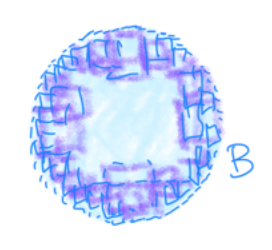
\includegraphics[scale=0.3]{images/base_rn} 
    \end{center}
    Pero también,
    \begin{center}
        
\includegraphics[scale=0.3]{images/bases_alternativas_rn} 
    \end{center}
    porque
    \[
    B\left( x, \varepsilon \right) = \bigcup_{i \in  I} cuadrados = \bigcup_{j \in J} rectangulos
    \]
\end{enumerate}
\end{ej}

\underline{Política general} , como antes: a menudo basta considerar los abiertos de $\mathcal{B}$ 

Ilustración: $A \subset X$ denso $\Leftrightarrow \forall B \in \mathcal{B}, B \cap A \neq \emptyset$.

\begin{prop}
$\mathcal{B} \subset \mathcal{P} \left( X \right)$ es base de una topología (única) $\mathcal{T}$ es $X$. Es equivalente a: 
\begin{itemize}
    \item $X = \bigcup_{B \in \mathcal{B}} B$.
    \item $\forall x \in B_1 \cap B_2,\ \exists B^x \subset B_1 \cap B_2$.
\end{itemize}
\begin{center}
    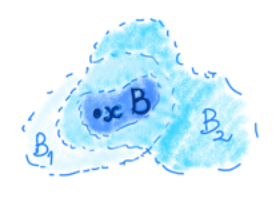
\includegraphics[scale=0.3]{images/base_unica} 
\end{center}
\end{prop}
\begin{demo}
\begin{itemize}
    \item \underline{Unicidad}: $\mathcal{T} = \{\bigcup_{i \in  I} B_i: \{B_i\} \subset \mathcal{B}\}$.
    \item \underline{Existencia}: Esa $\mathcal{T}$ es efectivamente topología. Lo importante: $B_1, B_2 \in \mathcal{B} \Rightarrow B_1 \cap B_2 = \bigcup_{x \in B_1 \cap B_2} B^x \in \mathcal{T}$.
\end{itemize}
\end{demo}

\section{Topología relativa}%
\label{sec:topologia_relativa}
Sea $\left( X, \mathcal{T} \right)$ espacio topológico.
\begin{defi}
$Y \subset X: \mathcal{T}|_Y = \{U \cap Y: U \in \mathcal{T}\}$ es una topología en $Y$ (fácil), denominada \underline{relativa} ó \underline{restricción} a $Y$; también se dice que $\left( Y, \mathcal{T}|_Y \right)$ es un \underline{subespacio} de $\left( X, \mathcal{T} \right)$ y que $\left( X, \mathcal{T} \right)$ es el espacio \underline{ambiente}. 
\begin{center}
    %TODO: Recortar mejor por arriba
    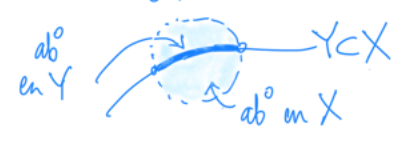
\includegraphics[scale=0.3]{images/def_subespacio_top} 
\end{center}
\end{defi}

\begin{obs}
\begin{enumerate}
    \item Los cerrados en $\mathcal{T}|_Y$ son $F\cap Y$ con $F$ cerrado en $\mathcal{T}$.
    \[
    \left[ Y \setminus U \cap Y = Y \cap \left( X \setminus U \right) = Y\cap F \right] 
    \]
    \item 
    $\begin{cases}
        y \in Y \subset X\\
        \mathcal{V}^y \text{ base de entornos de } y \text{ en } \mathcal{T} 
    \end{cases}\Rightarrow \begin{cases}
        \mathcal{V}^y \cap Y = \{V^y \cap Y : V^y \in \mathcal{V}^y\} \\
        \text{base de entornos de } y \text{ en } \mathcal{T}|_Y 
    \end{cases}$

    \item $\mathcal{B}$ base de $\mathcal{T} \Rightarrow \mathcal{B} \cap Y = \{B \cap Y : B \in \mathcal{B}\}$ base de $\mathcal{T}|_Y$
\end{enumerate}
\end{obs}

Esta idea es general: en un subespacio se hacen las construcciones intersecando.

\begin{ej}
\begin{enumerate}
    \item $y$ es un punto aislado de $Y \Leftrightarrow \{y\}$ abierto en $\mathcal{T}|_Y. \left[ \{y\} = V^y \cap Y \right]$
    \item Todos los puntos de $Y$ son aislados $\Leftrightarrow C|_Y = $ discreta.

    Se dice: $Y$ es un \underline{subespacio discreto}. 

    Por ejemplo, en $\mathbb{Z} \subset \mathbb{R}$:
    \begin{center}
        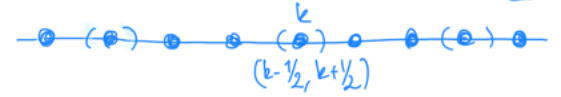
\includegraphics[scale=0.3]{images/def_subespacio_discreto} 
    \end{center}

    \item $a \in X, \mathcal{T}_a|_{X \setminus \{a\}} = $ discreta.
\end{enumerate}
\end{ej}

\begin{obs}
\begin{enumerate}
    \item $Y \subset_{\text{ab}} X: W \text{ abierto de } Y \Leftrightarrow W \text{ abierto de } X$ contenido en $Y$.
    \[
    \left[ W = U \cap Y^{\text{ab}},\ U^{\text{ab}} \subset X \Rightarrow W^{\text{ab}} \subset X \text{ por intersección finita} \right] 
    \]
    \item $Y \subset_{\text{cerr}} X: F \text{ cerrado de } Y \Leftrightarrow F \text{ cerrado de } X$ contenido en $Y$.
    \[
    \left[ C = F \cap Y^{\text{cerr}},\ F^{\text{cerr}} \subset X \Rightarrow C^{\text{cerr}} \subset X \text{ por intersección finita} \right] 
    \]
\end{enumerate}
\end{obs}

\chapter{Aplicaciones continuas}%
\label{cha:aplicaciones_continuas}
\section{Continuidad}%
\label{sec:continuidad}
El famoso $\varepsilon-\delta$ en $\mathbb{R}^n \mathcal{T}_u; x_0 \in X,\ f : \overbrace{X}^{\subset \mathbb{R}^p} \rightarrow \overbrace{Y}^{\subset \mathbb{R}^q}$: 
\begin{gather*}        
\forall \varepsilon > 0, \exists \delta > 0: 
\begin{cases}
    \lVert x - x_0 \rVert < \delta \Rightarrow \lVert f\left( x \right) - f\left( x_0 \right) \rVert < \varepsilon \Leftrightarrow\\
    x \in B\left( x_0, \delta \right) \Rightarrow f\left( x \right) \in B\left( f\left( x_0 \right), \varepsilon \right) \Leftrightarrow\\
    f\left( B\left( x_0, \delta \right) \right) \subset B\left( f\left( x_0 \right), \varepsilon \right) 
\end{cases} \Rightarrow\\
\boxed{\forall B\left( f\left( x_0 \right), \varepsilon \right),\ \exists B\left( x_0, \delta \right) \subset f^{-1}\left( B\left( f\left( x_0 \right), \varepsilon \right) \right)} 
.\end{gather*}

\begin{defi}
$f: X \rightarrow Y$ será \underline{continua en $x_0$} $\in X$ si: 
\[
\forall V^{f\left( x_0 \right)}: f^{-1}\left( V^{f\left( x_0 \right)} \right) = V^{x_0} 
\]
\end{defi}

\begin{prop}[Composición de continuidades]
La composición de funciones continuas es continua:

\[
X \xrightarrow{f} Y \xrightarrow{g} Z: \begin{rcases}
    f \text{ continua en } x_0\\
    g \text{ continua en } y_0
\end{rcases} \Rightarrow h = g \circ f \text{ continua en }  x_0
\]
\end{prop}
\begin{demo}
Sea $V^{h\left( x_0 \right)} \rightarrow h^{-1} V^{h\left( x_0 \right)} = f^{-1}g^{-1}V^{g\left( y_0 \right)} = f^{-1} V^{y_0} = V^{x_0}$.
\end{demo}

\begin{ej}
\begin{enumerate}
    \item $\forall f: X_{\text{discreta}} \rightarrow Y$ es continua. [Todo es abierto, luego todo es entorno en $\mathcal{T}_{\text{disc}}$]
    \item $\forall f: X \rightarrow Y_{\text{trivial}}$ continua. [$V^{f\left( x \right)} = Y$ es el único abierto, luego el único entorno, de $f^{-1}V^{f\left( x \right)} = f^{-1}Y = X$ es abierto]
    \item $f: X \rightarrow Y_{\text{discreta}}$ es continua $\Rightarrow f$ localmente creciente.
        [$\{f\left( x_0 \right)\} = V^{f\left( x_0 \right)}$ en $\mathcal{T}_{\text{discr}} \xRightarrow[f\text{ cont.}]{} f^{-1}f\left( x_0 \right) = V^{x_0}\; \land \;f \equiv f\left( x_0 \right)$]
    \item $f: X \rightarrow Y$ localmente constante $\Rightarrow$ continua.

    [$\forall x_0 \in X, \exists U^{x_0} : f \stackrel{U^{x_0}}{\equiv} f\left( x_0 \right) \Rightarrow \forall V^{f\left( x_0 \right)}: f^{-1}V^{f\left( x_0 \right)} \supset U^{x_0} \Rightarrow f^{-1}V^{f\left( x_0 \right)} = V^{x_0}$ es entorno de $x_0$]
\end{enumerate}
\end{ej}

\begin{prop}
Son equivalentes:
\begin{enumerate}
    \item $f$ es continua.
    \item $f^{-1}\left( \text{abierto}  \right) = \text{abierto} ,\ \forall \text{abierto} \in Y$.
    \item $f^{-1}\left( \text{cerrado} \right) = \text{cerrado},\ \forall $ cerrado de $Y$.
    \item $f^{-1}\left( \mathring{A} \right) \subset \inter\left( f^{-1}\left( A \right) \right),\ \forall A \subset Y$
    \item $f\left( \overline{A} \right) \subset \overline{f\left( A \right)},\ \forall A \subset X$
\end{enumerate}
\end{prop}
\begin{demo}
\begin{enumerate}
    \item $1 \Rightarrow 2)$
    \[
        W^{\text{ab}} \subset Y \Rightarrow W \text{ ent. de } f\left( x \right),\ \forall x \in f^{-1}W \Rightarrow f^{-1} W \text{ ent. de } \forall x \in f^{-1}W \Rightarrow f^{-1} W \subset X 
    \]
    \item $2 \Rightarrow 3)$
    \[
        C_{\text{cerr}} \subset Y \Rightarrow Y \setminus C \subset Y \Rightarrow^{2)} \underbrace{f^{-1}\left( Y\setminus C \right)}_{= X \setminus f^{-1}C} \subset X \Rightarrow f^{-1}C \stackrel{\text{cerr}}{\subset} X 
    \]
    \item $3 \Rightarrow 5)$

    \[
        \overline{f\left( A \right)} \stackrel{\text{cerr}}{\subset} Y \Rightarrow^{3)} \underbrace{f^{-1}\overline{f\left( A \right)}}_{\subset f^{-1}f\left( A \right) \supset A} \subset X \Rightarrow \overline{A} \subset f^{-1}\overline{f\left( A \right)} \Rightarrow f\left( \overline{A} \right) \subset \overline{f\left( A \right)} 
    \]
    \item $5 \Rightarrow 4)$
    \begin{gather*}
        Y \setminus \mathring{A}\Rightarrow \overline{Y\setminus A} \supset \overline{f\left( X \setminus f^{-1}A \right)} \stackrel{5)}{\supset} f\left( \overline{X \setminus f^{-1}\left( A \right)} \right) = f\left( X \setminus \inter\left( f^{-1}A \right) \right) \Rightarrow\\
        X \setminus \inter\left( f^{-1}A \right) \subset f^{-1}\left( Y\setminus \mathring{A} \right) = X \setminus f^{-1}\left( \mathring{A} \right)\Rightarrow f^{-1}\left( \mathring{A} \right) \subset \inter\left( f^{-1}A \right) 
    .\end{gather*}

    \item $4 \Rightarrow 1)$
    \begin{gather*}
        V^{f\left( x \right)} \Rightarrow f\left( x \right) \in \inter\left( V^{f\left( x \right)} \right) \Rightarrow x \in f^{-1}\left( \inter\left( V^{f\left( x \right)} \right) \right) \subset \inter\left( f^{-1}V^{f\left( x \right)} \right) \Rightarrow \\
        f^{-1}V^{f\left( x \right) } \text{ entorno de } x.
    \end{gather*}
\end{enumerate}
\end{demo}

\begin{obs}
\begin{enumerate}
    \item Los cuatros primeros enunciados tratan sobre ``imágenes inversas''. Por ejemplo, la segunda dice que $f^{-1}\mathcal{T}_Y \subset \mathcal{T}_X$.
    \item Pensando que un punto adherente es un ``punto límite'', $5$ nos dice que ``la imagen del límite es el límite de la imagen''.
    \item $Id: \left( X, \mathcal{T}_1 \right) \rightarrow \left( X, \mathcal{T}_2 \right)$ es continua $\Rightarrow \mathcal{T}_2 \subset \mathcal{T}_1$. [$Id^{-1}\mathcal{T}_1 = \mathcal{T}_2]$
\end{enumerate}
Y no mencionamos todos los ejemplos conocidos en espacios afines $\mathbb{R}^n$ con $\mathcal{T}_u$.
\end{obs}

\section{Continuidad y subespacios}%
\label{sec:continuidad_y_subespacios}
\begin{prop}
Sea $f: X \rightarrow Y$ continua y $Z \subset X$ subespacio $\Rightarrow f|_Z : Z \rightarrow Y$ es continua.
\end{prop}
\begin{demo}
Se aplica el criterio ``imagen inversa de abierto es abierto'' y la fórmula:
\[
\left( f|_Z \right)^{-1} \left( A \right) = Z \cap f^{-1}A,\ \forall A \subset Y
\]
\end{demo}

\underline{Criterios de continuidad por recubrimientos.} Sea $f: X \rightarrow Y$. 
\begin{itemize}
    \item \textbf{Por abiertos:} $\exists X = \bigcup_{i \in  I} U_i: \forall f|_{U_i} : U_i \rightarrow Y$ es continua. 

    \begin{demo}
    $W \subset Y \Rightarrow$
    \[
    \begin{cases}
        f^{-1}W = \bigcup_{i \in  I} U_i \cap f^{-1} W = \bigcup_{i \in  I} \left( f|_{U_i} \right)^{-1} W\\
        \left( f|_{U_i} \right)^{-1}W \subset U_i \subset X \Rightarrow \left( f|_{U_i} \right)^{-1} W \subset X
    \end{cases}\Rightarrow f^{-1}W \subset X  
    \]
    Por unión de abiertos.
    \end{demo}

    \item \textbf{Por cerrados:} $\exists X = \underbrace{\bigcup_{i \in  I}}_{\text{finita}} F_i: \forall f|_{F_i} : F_i \rightarrow Y$ es continua. 

    \begin{demo}
    $C \subset Y \Rightarrow$
    \[
    \begin{cases}
        f^{-1}C = \bigcup_{i \in  I} F_i \cap f^{-1} C = \bigcup_{i \in  I} \left( f|_{F_i} \right)^{-1} C\\
        \left( f|_{F_i} \right)^{-1}C \subset F_i \subset X \Rightarrow \left( f|_{F_i} \right)^{-1} C \subset X
    \end{cases}\Rightarrow f^{-1}C \subset X  
    \]
    Por unión finita de cerrados.
    \end{demo}
\end{itemize}

\section{Homeomorfismos}%
\label{sec:homeomorfismos}
Recordemos las definiciones de continuidad que hemos visto:
\[
f \text{ continua} \Leftrightarrow f^{-1}\left( \text{abierto} \right) = \text{abierto} \Leftrightarrow f^{-1}\left( \text{cerrado} \right) = \text{cerrado} 
\]
Ahora veamos que ocurre al invertir la relación.
\begin{defi}
Sea $f: X \rightarrow Y$, será $\begin{cases}
    \text{\underline{abierta}} \\
    \text{\underline{cerrada}} 
\end{cases} \Leftrightarrow \begin{cases}
    f\left( \text{ab} \right) = \text{ab}\\
    f\left( \text{cerr} \right) = \text{cerr} 
\end{cases} $    
\end{defi}

\begin{obs}
Cuidado continuidad no implica que sea abierta, cerrada ni viceversa.
\end{obs}

\begin{ej}
\begin{enumerate}
    \item $Id: X_{\text{trivial}} \rightarrow X_{\text{discreta}}$, -cont. +ab. +cerr.
    \item $Id: X_{\text{discreta}} \rightarrow X_{\text{trivial}}$, +cont. -ab. -cerr.
    \item $j: \left[ 0, 1 \right] \subset \mathbb{R}_{u}$, +cont. -ab. +cerr.
    \item $j: \left( 0, 1 \right) \subset \mathbb{R}_u$, +cont. +ab. -cerr.
\end{enumerate}
\end{ej}

\begin{prop}[Trivialidades esenciales]
Sea $f$ biyectiva es equivalente:
\begin{itemize}
    \item $f$ es abierta
    \item $f$ es cerrada
    \item $f^{-1}$ es continua.
\end{itemize}
\end{prop}
\begin{demo}
\begin{enumerate}
    \item $F_{\text{cerr}} \subset X \Rightarrow X\setminus F_{\text{ab}} \subset X \Rightarrow^{ f\text{ ab}} \underbrace{f\left( X\setminus F \right)}_{= Y\setminus f\left( F \right) \text{(biy.)}} \subset_{\text{ab}} X \Rightarrow f\left( F \right) \subset_{\text{cerr}} Y \Rightarrow f$ cerr.

    \item $F_{cerr} \subset X \Rightarrow^{f \text{cerr}} \underbrace{f\left( F \right)}_{= \left( f^{-1} \right)^{-1} \left( F \right) \text{(biy)}} \subset_{\text{cerr}} Y \Rightarrow f^{-1}$ cont.

    \item $U_{\text{ab}} \subset X \Rightarrow^{f^{-1} \text{cont}} \underbrace{\left( f^{-1} \right) ^{-1} \left( U \right) }_{f\left( U \right) \text{(biy.)}} \subset Y \Rightarrow f$ ab.
\end{enumerate}
\end{demo}

\begin{defi}
    Sea $f: X \rightarrow Y$ biyectiva, es \underline{homeomorfismo} si $f\ \&\ f^{-1}$ son continuas, o equivalentemente si:
    \[
    \begin{cases}
        f \text{ biy.}\\
        \text{cont.}\\
        \text{ab.} 
    \end{cases} \Leftrightarrow \begin{cases}
        f \text{ biy.}\\
        \text{cont.}\\
        \text{cerr.}
    \end{cases} 
    \]
\end{defi}

\begin{defi}[Localización de un homeomorfismo]
Sea $f: X \rightarrow Y$, es \underline{homeomorfismo local} en $x_0 \in X$ si $f: V^{x_0} \rightarrow V^{f\left( x_0 \right)}$ es homeomorfismo para entornos de $x_0$ y $f\left( x_0 \right)$. Se suele decir para entornos ``suficientemente pequeños''.
\end{defi}

\underline{Ejercicio:} Se pueden tomar $V^{x_0}, V^{f\left( x_0 \right)}$ abiertos.

\begin{obs}
Un homeomorfismo local es abierto.
\end{obs}
\begin{demo}
    $U \subset_{\text{ab}} X \Rightarrow f\left( U \right)$ entorno $\forall y_0 = f\left(\overbrace{x_0}^{\in U}\right) \in f\left( U \right)$.
    Como $f$ hom. local $\Rightarrow f| : V^{x_0} \rightarrow V^{y_0}$ es hom. $\Rightarrow f\left( \overbrace{U \cap V^{x_0}}^{\ni y_0 = f\left( x_0 \right)} \right) \subset_{\text{ab}} V^{y_0} \Rightarrow f\left( \overbrace{U \cap V^{x_0}}^{\subset f\left( U \right)} \right)$ entorno de $y_0 \Rightarrow f\left( U \right)$ entorno de $y_0$.
\end{demo}

\begin{ej}[¡Importantes!]
\begin{enumerate}
    \item Proyección estéreo? $\mathbb{S}^{m} \setminus \{\text{punto}\} \rightarrow \mathbb{R}^m$ hom.
    \item Proyección exponencial $\mathbb{R} \rightarrow \mathbb{S}': \theta \mapsto e^{2\pi i\theta} = \left( \cos 2\pi \theta, \sin 2\pi \theta \right)$, hom. local.
    \item Proyección antipodal: $\mathbb{S}^m \rightarrow \mathbb{R}P^{m}: x \mapsto \left[ x \right]$ hom. local.
    \item Lemniscata: $f: \mathbb{R} \rightarrow X \subset \mathbb{R}^2: t \mapsto \left( \frac{t}{1 + t^4}, \frac{t^3}{1 + t_4} \right)$ es biy. cont, pero \underline{no} hom. local.

    %TODO: Dibujo Lemniscata
    Engañosamente: 
    \[
        \forall t \in \mathbb{R} \exists \left( t - \varepsilon, t + \varepsilon \right) = I_{\varepsilon}: f| : I_{\varepsilon} \rightarrow f\left( I_{\varepsilon} \right) 
    \]
    es hom.

    En $t = 0, f\left( I_{\varepsilon} \right)$ \underline{no} es entorno de $f\left( 0 \right) = \left( 0, 0 \right)$.
\end{enumerate} 
\end{ej}

\begin{defi}
Una \underline{variedad topológica} de $\dim m$ es un espacio localmente homeomorfo a $\mathbb{R}^m$, es decir, cada punto tiene un entorno abierto homeomorfo a una bola $B\left( 0, \varepsilon \right) \subset \mathbb{R}^m$ (luego a cualquier bola, luego a todo $\mathbb{R}^m$).
\end{defi}

\chapter{Construcciones}%
\label{cha:construcciones}
\section{Imágenes inversas}%
\label{sec:imagenes_inversas}
\underline{Problema:} Hacer $f: Y \rightarrow \left( X, \mathcal{T} \right)$ continua con $\begin{cases}
    \text{top. discreta en } Y \text{ (matricialidad)}\\
    \text{top. \underline{menos fina} en } Y 
\end{cases}$ 

\underline{Sol:} $f^{-1} \mathcal{T} = \{f^{-1}U: U \in \mathcal{T}\}$ top. \underline{imagen inversa}. 
\begin{enumerate}
    \item Es topología (inm.)
    \item Es mínima. [$f$ es continua $\Rightarrow \forall f^{-1}U$ es abierto]
\end{enumerate}


%TODO: Fix teorema
\begin{theo}[Caracterización imagen inversa]
\begin{enumerate}
    \item
    \[
    \mathcal{T}' = f^{-1}\mathcal{T} \Leftrightarrow  
    \]
    \begin{equation}
        \forall g \left[ g \text{ cont.} \Leftrightarrow f \circ g \text{ cont.} \right]
    \end{equation}

    \item Y.
    %TODO: Fix composición
    \begin{center}
        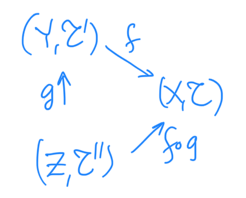
\includegraphics[scale=0.3]{images/caracterizacion_img_inv} 
    \end{center}
\end{enumerate}
\end{theo}
\begin{demo}
\begin{enumerate}
    \item $\mathcal{T}' = f^{-1}\mathcal{T}: $ 
    \begin{itemize}
        \item $g$ cont. $\Rightarrow f \circ g$ cont. (Composición de continuas)
        \item $f \circ g$ cont. $\Rightarrow g$ cont. ($V \in \mathcal{T}' \Rightarrow g^{-1}V \stackrel{\mathcal{T}' = f^{-1}\mathcal{T}}{=} g^{-1} f^{-1}U = \left( f \circ \right)^{-1} U \stackrel{f \circ g \text{ cont.}}{\in} \mathcal{T}''$)
    \end{itemize}

    \item Por otro lado,
    %TODO: Fix
    \begin{center}
        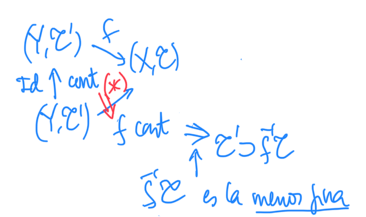
\includegraphics[scale=0.4]{images/dem_carac_img_inv_1} 
        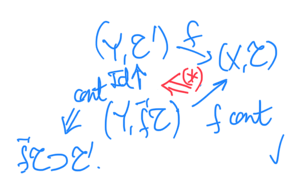
\includegraphics[scale=0.4]{images/dem_carac_img_inv_2} 
    \end{center}
\end{enumerate}
\end{demo}

\underline{Ejercicio}: Demostrar (ii) sin usar que $f^{-1}\mathcal{T}$ es la menos fina (usar que cumple la caracterización).

La anterior caracterización se llama \underline{propiedad universal}.

Caso esencial: 
\[
\boxed{f: Y \rightarrow X \text{ inyectiva}} 
\]

\begin{defi}
Una aplicación continua \underline{inyectiva} $f: \left( Y, \mathcal{T}' \right) \rightarrow \left( X, \mathcal{T} \right)$ tal que $\mathcal{T}' = f^{-1} \mathcal{T}$ se llama \underline{inmersión} (se suelen omitir las topologías).
\end{defi}

\begin{obs}
\begin{enumerate}
    \item $\mathcal{T}' = f^{-1}\mathcal{T} \Leftrightarrow \left( Y, \mathcal{T}' \right) \xrightarrow{\text{hom.}} \left( f\left( Y \right), \mathcal{T}|_{f\left( Y \right)} \right)$
    \[
    [V \in f^{-1}\mathcal{T} \Leftrightarrow V = f^{-1}\underbrace{U}_{\mathcal{T}} = f^{-1}\left( \underbrace{U \cap f\left( Y \right)}_{\mathcal{T}\mid f\left( Y \right)} \right)] 
    \]

    \item $f: Y \rightarrow X$ $1-1$ cont. $+ \begin{cases}
        \text{ab. } \Rightarrow \text{inmersión } [\text{ab. en } X \Rightarrow \text{ab. en } f\left( Y \right)\\
        \text{cerr.} \Rightarrow \text{inmersión } [\text{cerr. en } X \Rightarrow \text{cerr. en} f\left( Y \right)] 
    \end{cases} $
    \[
    \begin{cases}
        f\left( Y \right) \stackrel{\text{ab.}} X: V = f^{-1}U \in f^{-1}\mathcal{T} \Rightarrow fV = U \cap f\left( Y \right) \in \mathcal{T} \left( \text{inter. abierto} \right)\\
        f\left( Y \right) \stackrel{\text{cerr.}} X: C \text{ c.} f^{-1}\mathcal{T} \Rightarrow Y\setminus C = f^{-1} U \in f^{-1}\mathcal{T} \Rightarrow f\left( C \right) \left( X\setminus U \right) \cap f\left( Y \right) \stackrel{\text{cerr.}}{\subset} X \text{ i. c.} 
    \end{cases} 
    \]

    \item Tenemos: 
    \begin{itemize}
        \item Inmersión $ + \not$ ab. $+ \not$ cerr.
        \item Inmersión $+$ ab. $+ \not $ cerr.
        \item Inmersión $+$ ab. $+$ cerr.
    \end{itemize}
\end{enumerate}
\end{obs}

\begin{obs}
Las inmersiones permiten considerar unos espacios como subespacios de otros. Las frases ``el plano proyectivo real no es un subespacio de $\mathbb{R}^3$'', ``la esfera no es un subespacio de $\mathbb{R}^2$'', ``el plano proyectivo real es un subespacio de $\mathbb{R}^4$'' se refieren a esto: \underline{cuándo hay o no hay} una inmersión del primer espacio en el segundo, es decir, un subespacio del segundo homeomorfismo al primero. Es un problema fundamental de la topología
y de la geometría.
\end{obs}

\section{Imágenes directas}%
\label{sec:imagenes_directas}
\underline{Problema:} Hacer $f: \left( X, \mathcal{T} \right) \rightarrow Y$ continua en $\begin{cases}
    \text{top. trivial en } Y \text{(matrivialidad)}\\
    \text{top. \underline{más fina} en } Y 
\end{cases} $ 

\underline{Sol:} $f\mathcal{T} = \{V \subset Y: f^{-1}V \in \mathcal{T}\}$ top. \underline{imagen directa}.
\begin{enumerate}
    \item Es topología (inm.)
    \item Máxima [$f$ es continua $\Leftrightarrow \forall f^{-1} V$ es abierto] 
\end{enumerate}

\begin{theo}[Caracterización imágenes directas]
\begin{enumerate}
    \item
    \[
    \mathcal{T}' = f\mathcal{T} \Leftrightarrow  
    \]
    \begin{equation}
        \forall g \left[ g \text{ cont.} \Leftrightarrow g \circ f \text{ cont.} \right]
    \end{equation}

    \item Y.
    %TODO: Fix composición
    \begin{center}
        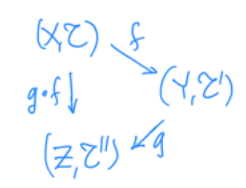
\includegraphics[scale=0.3]{images/caracterizacion_img_dir} 
    \end{center}
\end{enumerate}
\end{theo}
\begin{demo}
\begin{enumerate}
    \item $\mathcal{T}' = f^{-1}\mathcal{T}: $ 
    \begin{itemize}
        \item $g$ cont. $\Rightarrow g \circ f$ cont. (Composición de continuas)
        \item $g \circ f$ cont. $\Rightarrow g$ cont. ($W \in \mathcal{T}'' \Rightarrow f^{-1}\left( g^{-1} W \right) = \underbrace{\left( g \circ f \right)}_{\text{cont.}}^{-1} W \in \mathcal{T} \stackrel{\mathcal{T}' = f\mathcal{T}}{\Rightarrow} g^{-1}W \in \mathcal{T}'$)
    \end{itemize}

    \item Por otro lado,
    %TODO: Fix
    \begin{center}
        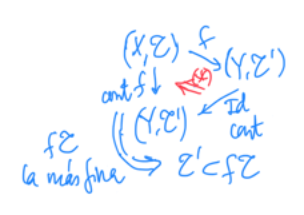
\includegraphics[scale=0.4]{images/dem_carac_img_dir_1} 
        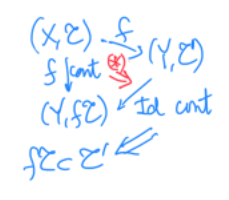
\includegraphics[scale=0.4]{images/dem_carac_img_dir_2} 
    \end{center}
\end{enumerate}
\end{demo}

\underline{Ejercicio}: Demostrar (ii) sin usar que $f\mathcal{T}$ es la más fina (usar que cumple la caracterización)

La caracterización anterior se llama \underline{propiedad universal}.

\begin{obs}
$f\left( X \right)$ es abierto y cerrado en $f\mathcal{T}: \begin{cases}
    \forall y \in Y \setminus f\left( X \right), f^{-1}y = \emptyset \in \mathcal{T} \Rightarrow \{y\} \in f\mathcal{T}\\
    f^{-1}f\left( X \right) = X \in \mathcal{T} \Rightarrow f\left( X \right) \in f\mathcal{T}
\end{cases}$
\end{obs}

Caso esencial:
\[
\boxed{f: X \rightarrow Y \text{ sobreyectiva}.} 
\]
Para entender los abiertos de una imagen directa es conveniente representarlos en el dominio. El concepto es conjuntista en realidad:

\begin{defi}
Un conjunto $A \subset X$ es \underline{saturado} (respecto de $f$) si $f^{-1}f\left( A \right) = A$.
\end{defi}
\begin{prop}
Los abiertos de $f\mathcal{T}$ son las imágenes de los abiertos saturados de $\mathcal{T}$.    
\end{prop}
\begin{demo}
\begin{enumerate}
    \item $V \in f\mathcal{T} \Rightarrow f^{-1}V \in \mathcal{T}$ y $V \stackrel{f \text{ sobre}}{=} f^{-1}fV$
    \item $U \in \mathcal{T}$, saturado $\Rightarrow f\left( U \right) = V \in f\mathcal{T}: f^{-1}V = f^{-1}f\left( U \right) \stackrel{U \text{ sat.}}{=} U \in \mathcal{T}$
\end{enumerate}
\end{demo}

\begin{obs}
Los abiertos \underline{no} saturados de $X$ pueden tener imágenes \underline{no} abiertas de $Y$. 
\end{obs}

\begin{ej}
\begin{enumerate}
    \item $f: \left[ 0, 1 \right] \rightarrow \mathbb{S}^1 = Y: t \mapsto \left( \cos 2\pi t, \sin 2\pi t \right) = \exp\left( 2 \pi i t \right)$
    %TODO: Fix image
    \begin{center}
        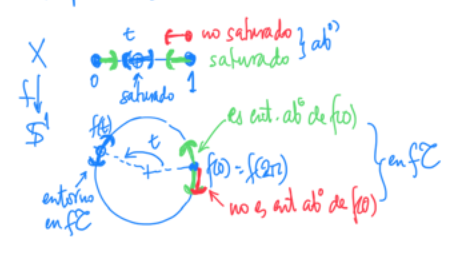
\includegraphics[scale=0.4]{images/ej_sat_1} 

        \textit{La topología imagen directa es la usual en $\mathbb{S}^1$.} 
    \end{center}

    \item Tenemos:
    \begin{align*}
        f: R = \left[ 0, 1 \right] \times \left[ 0, 1 \right] &\rightarrow C \subset \mathbb{R}^3: x^2 + y^2 = 1,\ 0 \le z \le 1\\
        \left( s, t \right) &\mapsto \left( \cos 2\pi s, \sin 2\pi s, t \right) 
    .\end{align*}

    %TODO: Fix image
    \begin{center}
        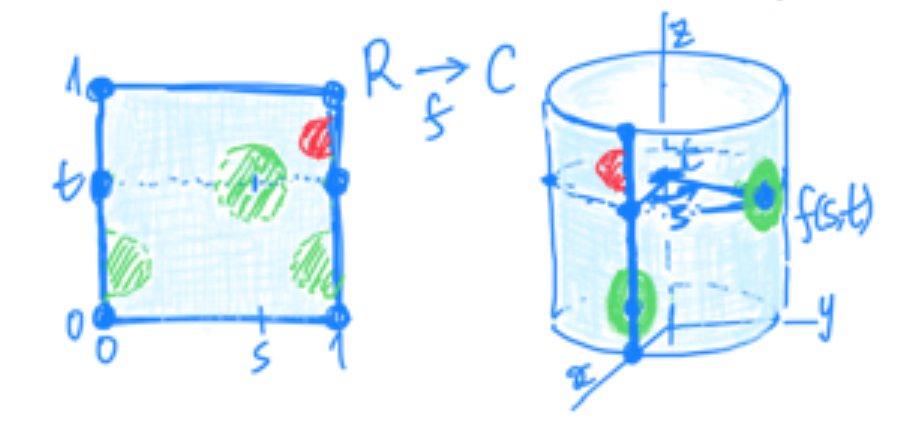
\includegraphics[scale=0.3]{images/ej_top_dir_2}

        \textit{Analizando los abiertos saturados y no saturados se concluye que la topología imagen directa es la usual en el tronco del cilindro.} 
    \end{center}
\end{enumerate}
\end{ej}

\begin{defi}
Una aplicación continua sobre $f: \left( X, \mathcal{T} \right) \rightarrow \left( Y, \mathcal{T}' \right)$ tal que $\mathcal{T}' = f\mathcal{T}$ se llama \underline{identificación} (se suelen omitir las topologías)
\end{defi}

\begin{obs}
\begin{enumerate}
    \item Identificación: $V \stackrel{\text{ab}}{\subset} Y \Leftrightarrow f^{-1}V \stackrel{\text{ab}}{\subset} X$

    Continua: $V \stackrel{\text{ab}}{\subset } Y \Rightarrow f^{-1}V \stackrel{\text{ab}}{\subset} X$

    \item Sea $f: X \rightarrow Y$ sobre. continua. Si además es:
    \begin{itemize}
        \item Abierta $\Rightarrow f$ es identificación [por (1)]
        \item Cerrada $\Rightarrow f$ es identificación [$f^{-1}V \stackrel{\text{ab}}{\subset} X \stackrel{\text{+ cerr.}}{\Rightarrow} f\left( \underbrace{X \setminus f^{-1}\left( V \right)}_{= Y\setminus V} \right) \stackrel{\text{cerr.}}{\subset} Y \Rightarrow V \stackrel{\text{ab}}{\subset} Y$
    \end{itemize}
\end{enumerate}
\end{obs}

\underline{Cocientes}: Caso particular: $\left( X, \mathcal{T} \right) \stackrel{p}{\rightarrow} Y = \underbrace{X / \sim}_{p \mathcal{T} = \text{top. cociente}}$. Cociente respecto de una relación de equivalencia en $X$. 
\begin{center}
    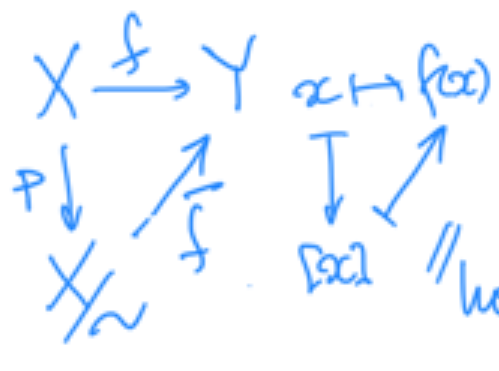
\includegraphics[scale=0.2]{images/def_cociente} 
\end{center}
Tenemos que $x_1 \sim x_2 \stackrel{\text{def}}{\Leftrightarrow} f\left( x_1 \right) = f\left( x_2 \right)$

\underline{Política general:} Los cocientes son cómodos para definir espacios, las identificaciones son mejores para estudiar las propiedades que tenemos. Conviene pues tener triángulos como el anterior. Se puede contemplar $Y$ como un modelo del cociente.

%TODO: Fix imágenes
\begin{ej}[Anteriores]
La circunferencia y el cilindro como cocientes:
\begin{center}
    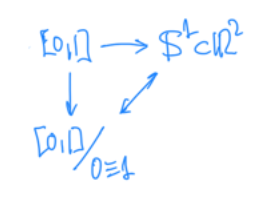
\includegraphics[scale=0.4]{images/ej_cociente_1} 
    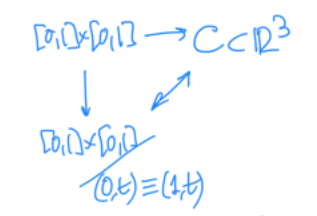
\includegraphics[scale=0.4]{images/ej_cociente_2}
\end{center}

Para representar cocientes se utilizan dibujos que indican las identificaciones en los espacios de partida:
\begin{center}
    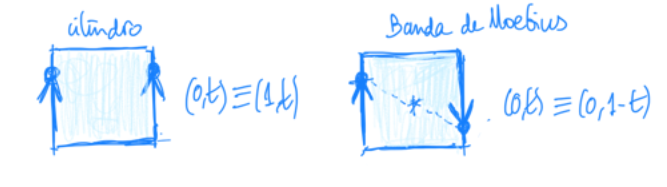
\includegraphics[scale=0.3]{images/ej_cociente_3} 
\end{center}
\end{ej}

\end{document}
